\hypertarget{mtk__robin__bc__descriptor__2d_8cc}{\section{src/mtk\+\_\+robin\+\_\+bc\+\_\+descriptor\+\_\+2d.cc File Reference}
\label{mtk__robin__bc__descriptor__2d_8cc}\index{src/mtk\+\_\+robin\+\_\+bc\+\_\+descriptor\+\_\+2d.\+cc@{src/mtk\+\_\+robin\+\_\+bc\+\_\+descriptor\+\_\+2d.\+cc}}
}


Impose Robin boundary conditions on the operators and on the grids.  


{\ttfamily \#include \char`\"{}mtk\+\_\+tools.\+h\char`\"{}}\\*
{\ttfamily \#include \char`\"{}mtk\+\_\+robin\+\_\+bc\+\_\+descriptor\+\_\+2d.\+h\char`\"{}}\\*
Include dependency graph for mtk\+\_\+robin\+\_\+bc\+\_\+descriptor\+\_\+2d.\+cc\+:
\nopagebreak
\begin{figure}[H]
\begin{center}
\leavevmode
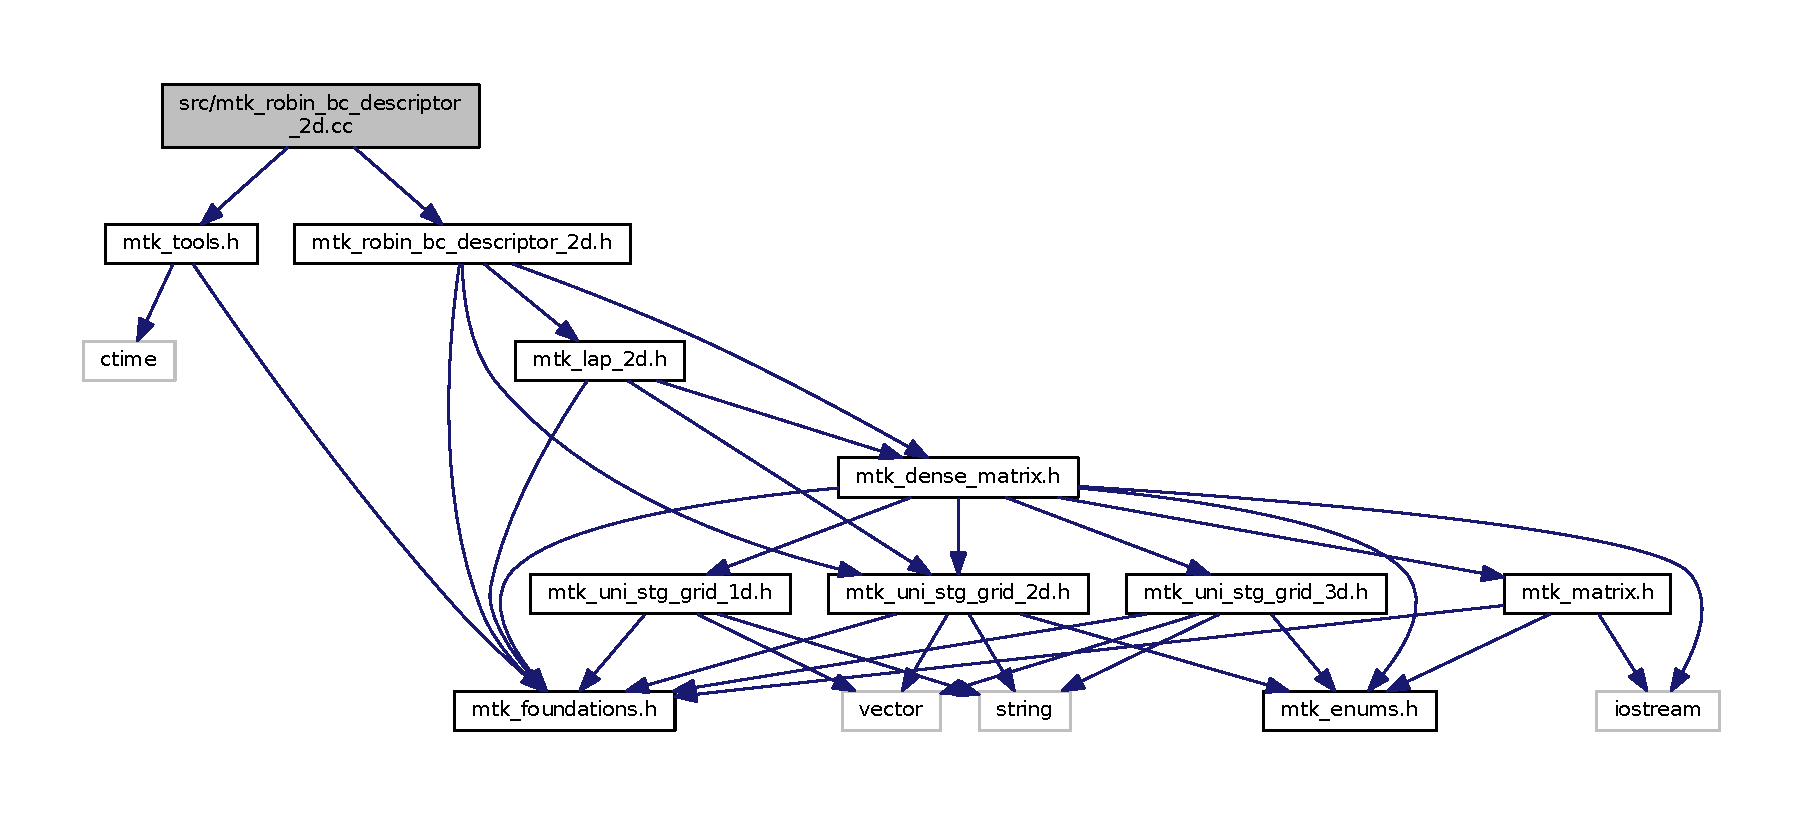
\includegraphics[width=350pt]{mtk__robin__bc__descriptor__2d_8cc__incl}
\end{center}
\end{figure}


\subsection{Detailed Description}
This class presents an interface for the user to specify Robin boundary conditions on 2\+D mimetic operators and the grids they are acting on.

{\bfseries Def.} Let $ u(\mathbf{x},t):\Omega\times [t_0, t_n]\mapsto\mathbb{R} $ be the solution to an ordinary or partial differential equation of interest. We say that $ u $ satisfies a {\bfseries Robin boundary condition on} $ \partial\Omega $ if and only if there exists $ \beta(\mathbf{x},t):\Omega\times [t_0, t_n]\mapsto\mathbb{R} $ so that\+: \[ \forall t \in [t_0,t_n]\; \forall \mathbf{x} \in \partial\Omega: \delta(\mathbf{x},t)u(\mathbf{x},t) + \eta(\mathbf{x},t)(\hat{\mathbf{n}}\cdot\nabla u) = \beta(\mathbf{x},t). \]

Intuitively, a {\bfseries Robin boundary condition} is a constraint that must be satisfied by any linear combination of any scalar field $ u $ and its first normal derivative, in order for $ u $ to represent a unique solution to a given ordinary or partial differential equation of interest.

Instances of this class receive information about the coefficient functions and each condition for any subset of the boundary (west, east, south and north in 2\+D). These instances then handle the complexity of placing the coefficients in the differentiation matrices and the conditions in the grids.

\begin{DoxySeeAlso}{See also}
\href{http://mathworld.wolfram.com/NormalVector.html}{\tt http\+://mathworld.\+wolfram.\+com/\+Normal\+Vector.\+html}
\end{DoxySeeAlso}
\begin{DoxyAuthor}{Author}
\+: Eduardo J. Sanchez (ejspeiro) -\/ esanchez at mail dot sdsu dot edu 
\end{DoxyAuthor}


Definition in file \hyperlink{mtk__robin__bc__descriptor__2d_8cc_source}{mtk\+\_\+robin\+\_\+bc\+\_\+descriptor\+\_\+2d.\+cc}.

